\chapter[Creación certificados digitales.]{Creación de los certificados digitales para la aplicación.}\label{cap:anexoB}
\markboth{ANEXO \ref{cap:anexoB}. CREACIÓN CERTIFICADOS DIGITALES.}{}

En este anexo vamos a explicar como hemos realizado la generación de los certificados digitales usados tanto por la aplicación del móvil, como las aplicación web para la verificación de las firmas.

El programa elegido fue XCA (\url{http://xca.sourceforge.net/}) que es un gestor de certificados y claves, implementado por Christian Hohnstädt. Se eligió dicho programa por ser multiplataforma, por lo que se podrían generar los certificados en cualquier sistema.

XCA está e los repositorios de Ubuntu, por lo que para instalarlo solo hay que proceder a su instalación normal. 

\begin{lstlisting}[style=consola]
sudo apt-get install xca
\end{lstlisting}

Para instalarlo en otro sistema se puede descargar desde: \url{http://sourceforge.net/projects/xca/}.

Una vez instalado, XCA proporciona una interfaz gráfica con la que realizar todo el proceso. Lo primero es generar la CA. Para ello pulsamos en File -> New Database. Elegimos donde queremos guardar toda la información. En el siguiente paso nos pedirá que establezcamos una contraseña para la CA (figura~\ref{fig:password}).

\begin{figure}
  \centering
    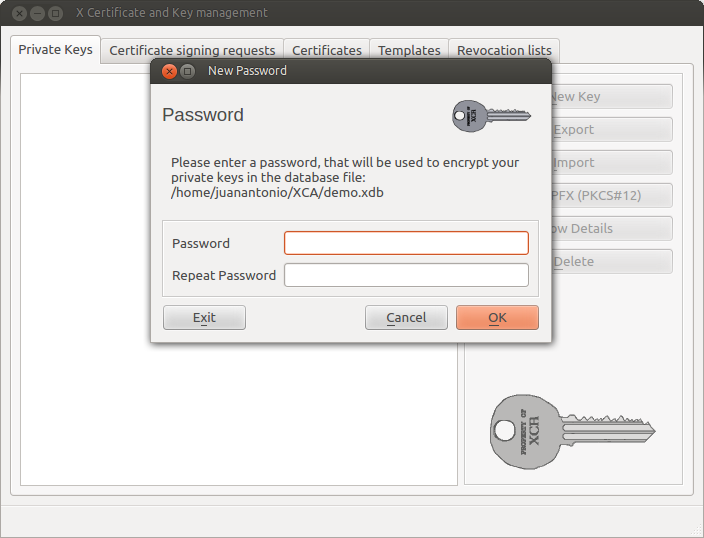
\includegraphics[scale=0.6]{./AnexoCreacionCertificado/imagenes/password.png}
  \caption{Password para la CA.}
  \label{fig:password}
\end{figure}

El siguiente paso sería generar el certificado que vamos a usar, para ello vamos a la pestaña Certificates y pulsamos New Certificate, en la nueva pantalla que se abre podemos rellenar los valores que necesitemos en la pestaña Subject y debemos generar una nueva clave privada pulsando en el botón de Generate a new key (figura\ref{fig:clavePrivada}). Una vez generada podemos definir los usos para los que queremos que se pueda usar el certificado en la pestaña Key usage.

\begin{figure}
  \centering
    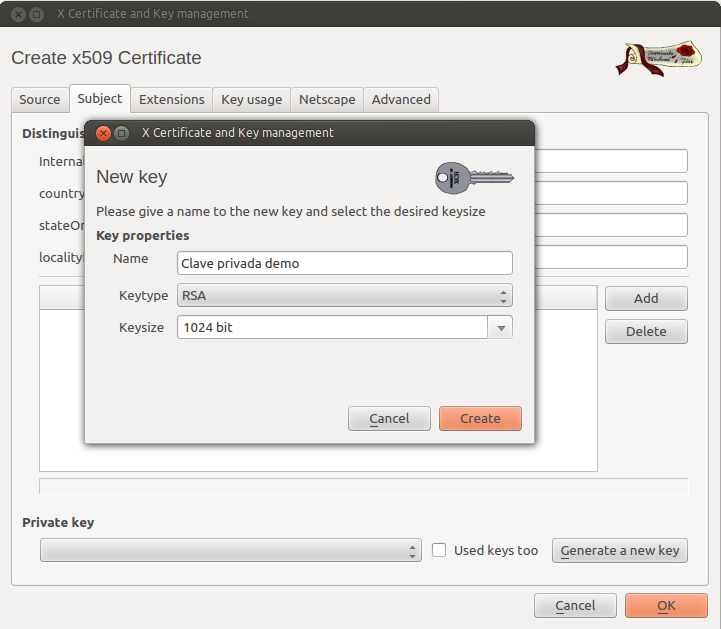
\includegraphics[scale=0.6]{./AnexoCreacionCertificado/imagenes/clavePrivada.png}
  \caption{Creación de la clave privada.}
  \label{fig:clavePrivada}
\end{figure}

Una vez generado el certificado lo exportamos en formato PKCS\#12 y lo almacenamos en la ruta que queramos (figura~\ref{fig:exportacion}).

\begin{figure}
  \centering
    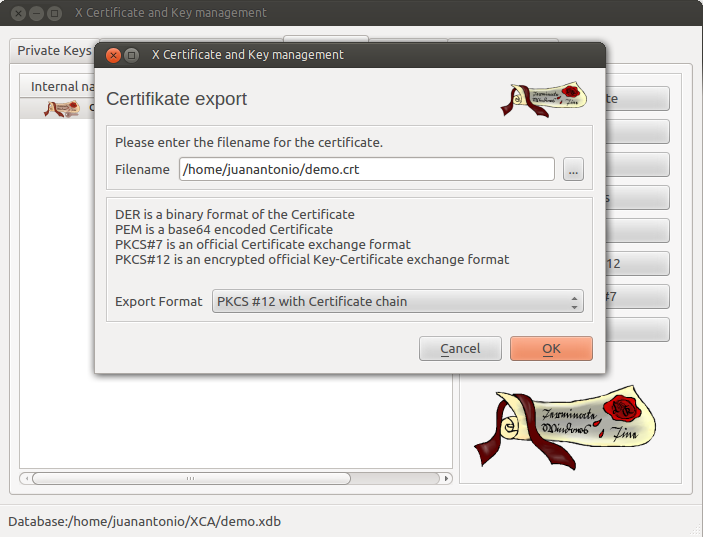
\includegraphics[scale=0.6]{./AnexoCreacionCertificado/imagenes/exportacion.png}
  \caption{Exportación del certificado.}
  \label{fig:exportacion}
\end{figure}

Una vez creado el archivo *.p12 debemos de meterlo en el móvil y subirlo a la aplicación web en la pestaña Añadir certificados. En el movil hay que colocarlo en el directorio que se configuró la primera vez que se ejecutó la aplicación.

En caso de que el proyecto se llevase a cabo en la realidad este proceso no podría hacerlo el usuario y debería haber un control exhaustivo de dichos certificados con listas de revocación, entidades que firmasen los certificados, etc.








